\chapter{White Dwarfs, Neutron Stars, and Strong-Field Physics}
\label{chap:e18}

\begin{chapteropening}
So far, the ``quantum light sources'' we have dealt with have mostly been ordinary stars: a ball of hot gas with a surface temperature of a few thousand to a few tens of thousands of kelvin, emitting broadband thermal light (Chapter~\ref{chap:e17}). This chapter walks to the terminal stations of stellar evolution: the white dwarf and the neutron star. They are two extreme specimens that place quantum physics directly in the sky: a white dwarf is held up against collapse by the electrons' \emph{Pauli exclusion principle}, and the magnetic field at a neutron star's surface can be strong enough to turn \emph{the vacuum itself} into a medium with a preferred polarization direction. But for us observers, who ``can only count photons, measure phases, and read polarization,'' they bring a very practical nuisance: they are far too small. A white dwarf is only the size of the Earth, and a neutron star only a dozen kilometers; placed tens to hundreds of parsecs away, their angular diameters are only microarcseconds, and no single-aperture telescope can hope to ``see them as a surface.'' So this chapter twines two threads together: one is \textbf{physics}: degeneracy pressure, magnetosphere, cyclotron radiation, vacuum birefringence, surface atmosphere; the other is \textbf{method}: since we cannot resolve the spatial structure, we switch to three rulers, time (phase folding), energy (spectra), and polarization (Stokes parameters), and compress the information about the compact object into the same event table. Both threads ultimately lead to the ``polarization quantum channel'' that Chapter~\ref{chap:e22} will open up specifically.
\end{chapteropening}


\section{White Dwarfs: How Electron Degeneracy Pressure Holds Up a Star}
\label{sec:e18-degeneracy}

Ask first the most naive question: a star has burned up its nuclear fuel, with no thermonuclear reaction pushing outward any longer: why does it not simply collapse all the way to a point? An ordinary star relies on ``thermal pressure'': the hotter the gas, the more fiercely the particles collide, and the greater the outward pressure. But a white dwarf has already cooled down, and thermal motion recedes to a secondary role. What truly holds up gravity is a pressure that \emph{does not vanish even when the temperature falls to zero}: electron degeneracy pressure. Its origin is purely quantum mechanical.

The physical picture is this. Think of the electrons in a white dwarf as a crowd of passengers confined in a box; the Pauli exclusion principle dictates that ``one seat (quantum state) holds at most one (two counting spin).'' The more you compress the box, the fewer low-energy seats there are to go around, and later electrons are forced into seats of \emph{very high momentum}. High momentum means moving fast and hitting the walls often, so even without any heating this crowd of electrons pushes hard outward. The higher the density, the higher the momentum they are pushed to, and the greater the pressure: this is degeneracy pressure.

Let us write it as a formula. First compute ``how full the seats are.'' In momentum space, the volume of the sphere of momentum less than \(p\) is \(\tfrac{4}{3}\pi p^3\); quantum mechanics tells us that each phase-space cell of volume \(h^3\) holds only two electrons (spin up and spin down). So the number density of electrons per unit volume, filled up to \(p_F\) (the Fermi momentum), is
\[
  n_e=\frac{2}{h^3}\cdot\frac{4}{3}\pi p_F^3
     =\frac{8\pi p_F^3}{3h^3}
     =\frac{p_F^3}{3\pi^2\hbar^3},
\]
the last step using \(h=2\pi\hbar\). Inverting for the Fermi momentum:

\begin{equation}
  p_F=\hbar\,(3\pi^2 n_e)^{1/3},
  \qquad
  n_e=\frac{\rho}{\mu_e m_p}.
  \label{eq:e18-fermi}
\end{equation}
\begin{formulaexplain}
\(p_F\): the Fermi momentum (\(\mathrm{g\,cm\,s^{-1}}\)), the highest momentum to which electrons are filled. \(n_e\): the electron number density (\(\mathrm{cm^{-3}}\)). \(\rho\): the mass density; \(\mu_e\): the number of baryons per electron (\(\simeq2\) for a carbon-oxygen star); \(m_p\): the proton mass. The higher the density, the higher the electrons are pushed by the Pauli principle.
\end{formulaexplain}

Grounding each symbol: the unit of \(n_e\) is \(\mathrm{cm^{-3}}\); \(\rho\) is the mass density (\(\mathrm{g\,cm^{-3}}\)); \(m_p=1.67\times10^{-24}\,\mathrm{g}\); \(\mu_e\) appears because a white dwarf contains both electrons and atomic nuclei, and on average each electron is ``paired'' with the mass of \(\mu_e\) nucleons, with carbon-oxygen composition giving approximately \(\mu_e\simeq2\). Plug in a real number: a typical DA white dwarf of \(M\simeq0.6\,M_\odot\) and radius about the size of the Earth (\(R\simeq0.012\,R_\odot\simeq1.3\,R_\oplus\)) already reaches a mean density of order \(10^6\,\mathrm{g\,cm^{-3}}\), rising to \(10^6\)--\(10^9\,\mathrm{g\,cm^{-3}}\) at the center. This density is a million times that of water: a teaspoon of such matter weighs a ton.

With \(p_F\) in hand we can compute the pressure. The pressure of an ideal Fermi gas comes from the momentum flux: \(P=\tfrac13\int_0^{p_F} v(p)\,p\,\dfrac{8\pi p^2}{h^3}\,dp\), where \(\tfrac13\) is the geometric factor for sharing over three directions and \(v(p)\) is the velocity of an electron of momentum \(p\). When the electrons move much slower than light (\(p_F\ll m_ec\)), \(v=p/m_e\), and the integral is
\[
  P_{\rm NR}=\frac{8\pi}{3h^3m_e}\int_0^{p_F}p^4\,dp
           =\frac{8\pi\,p_F^5}{15h^3m_e}
           =\frac{p_F^5}{15\pi^2\hbar^3 m_e}.
\]
Substituting the \(p_F\) of \(\eqref{eq:e18-fermi}\) and tidying up the exponents gives

\begin{equation}
  P_{\rm NR}=\frac{(3\pi^2)^{2/3}}{5}\,
             \frac{\hbar^2}{m_e}\,n_e^{5/3}.
  \label{eq:e18-pnr}
\end{equation}
\begin{formulaexplain}
\(P_{\rm NR}\): the non-relativistic electron degeneracy pressure (\(\mathrm{dyn\,cm^{-2}}\)), rising with density as \(n_e^{5/3}\). This is a ``very stiff'' support: a slight rise in density brings a sharp rise in pressure, and an ordinary white dwarf holds up gravity on it.
\end{formulaexplain}

Note that exponent \(5/3\). It means this pressure is ``very stiff'': try to compress it a bit more and it resists much harder. This is why low-mass white dwarfs can exist safely and stably for billions of years.

But as the mass grows, trouble comes. The larger the mass, the tighter it is compressed and the higher \(n_e\), and the Fermi momentum may exceed \(m_ec\): the electrons are pushed to \emph{near the speed of light}. Now \(v\to c\) is no longer \(p/m_e\); the velocity is capped at the speed of light and cannot rise further. Substituting \(v=c\) into the same pressure integral:
\[
  P_{\rm ER}=\frac{8\pi c}{3h^3}\int_0^{p_F}p^3\,dp
           =\frac{2\pi c\,p_F^4}{3h^3}
           =\frac{c\,p_F^4}{12\pi^2\hbar^3},
\]
then substituting \(p_F\):

\begin{equation}
  P_{\rm ER}=\frac{(3\pi^2)^{1/3}}{4}\,\hbar c\,n_e^{4/3}.
  \label{eq:e18-per}
\end{equation}
\begin{formulaexplain}
\(P_{\rm ER}\): the extreme-relativistic electron degeneracy pressure, with the density exponent softened to \(4/3\). Once the support softens, adding more mass makes the radius shrink sharply: this is the physical root of the approach to the Chandrasekhar limit.
\end{formulaexplain}

Now the exponent has fallen from \(5/3\) to \(4/3\). This drop is fatal: the response of pressure to density becomes ``softer,'' and adding more mass, it can no longer hold up much. In the extreme case, the density exponents of gravity and degeneracy pressure become equal, and the star loses its stable support: this is the physical origin of the Chandrasekhar limit (Chandrasekhar mass) \citep{1931ApJ....74...81C,1935MNRAS..95..207C,1961ApJ...134..683H}.

Connecting the above scaling relations to a form observers can use, one commonly writes Nauenberg's mass--radius approximation:

\begin{equation}
  R\simeq 0.0112\,R_\odot
  \left[\left(\frac{M_{\rm Ch}}{M}\right)^{2/3}
  -\left(\frac{M}{M_{\rm Ch}}\right)^{2/3}\right]^{1/2},
  \qquad
  M_{\rm Ch}\simeq 5.83\,\mu_e^{-2}\,M_\odot .
  \label{eq:e18-nauenberg}
\end{equation}
\begin{formulaexplain}
\(R\): the white-dwarf radius; \(M\): the mass; \(M_{\rm Ch}\): the Chandrasekhar limiting mass (about \(1.46\,M_\odot\) for \(\mu_e=2\)). As \(M\to M_{\rm Ch}\), the bracket tends to zero and the radius collapses toward zero: ``heavier means smaller.''
\end{formulaexplain}

This equation synthesizes the two pressures \(\eqref{eq:e18-pnr}\) and \(\eqref{eq:e18-per}\) into a single curve. It assumes zero temperature, no rotation, and no strong-field deformation, and is suited to estimating the main scaling of \(0.2\)--\(1.35\,M_\odot\) white dwarfs. Note its temperament, \emph{opposite} to that of ordinary stars: an ordinary star is larger when heavier, but a white dwarf is smaller when heavier. The true radius is further affected by core composition, the thickness of the hydrogen-helium envelope, finite temperature, and magnetic field, and high-precision work relies on evolutionary models or binary constraints \citep{1972ApJ...175..417N,2017MNRAS.470.4473P,2020ApJ...899..146C}. Figure~\ref{fig:e18-wd-mr} plots out this ``heavier means smaller'' curve.

\begin{figure}[tbp]
\centering
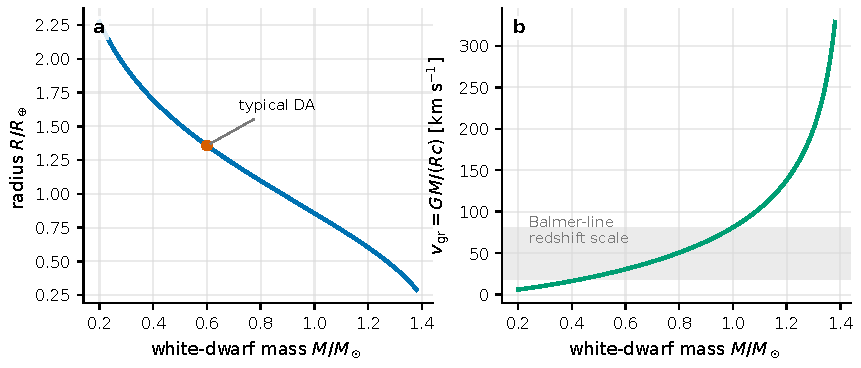
\includegraphics[width=0.94\linewidth]{figures/generated/chapter_11/ch11_white_dwarf_mass_radius.pdf}
\caption{As a white dwarf's mass increases its radius shrinks, contracting faster near the Chandrasekhar limit. The right panel converts the same mass--radius relation into the spectroscopically measurable gravitational-redshift velocity \(v_{\rm gr}=GM/(Rc)\); the Balmer-line redshift of a typical DA white dwarf is a few tens of \(\mathrm{km\,s^{-1}}\), already approaching or exceeding the velocity scale of ordinary stellar atmospheric motion.}
\label{fig:e18-wd-mr}
\end{figure}


\section{Small Angular Scale: Why Compact Objects Are So Hard to ``See Clearly''}
\label{sec:e18-angsize}

The previous section worked out that a white dwarf is only about the size of the Earth. This section translates this ``small'' into the quantity observers dread most: the angular diameter. Recall the definition from the imaging discussion of Chapter~\ref{chap:e11}: a disk of true diameter \(2R\) at distance \(d\) subtends an angle

\begin{equation}
  \theta_{\rm WD}=\frac{2R}{d}
  \simeq 11\,\mu\mathrm{as}
  \left(\frac{R}{0.012\,R_\odot}\right)
  \left(\frac{10\,\mathrm{pc}}{d}\right).
  \label{eq:e18-theta}
\end{equation}
\begin{formulaexplain}
\(\theta_{\rm WD}\): the white-dwarf angular diameter (microarcseconds \(\mu\mathrm{as}\)); \(R\): the radius; \(d\): the distance. Even as close as \(10\,\mathrm{pc}\), it is only about \(11\,\mu\mathrm{as}\), far beyond the resolving power of a single-aperture telescope.
\end{formulaexplain}

Lay out the numbers to feel it. \(1\,\mathrm{rad}=2.06\times10^{11}\,\mu\mathrm{as}\); \(10\,\mathrm{pc}=3.1\times10^{19}\,\mathrm{cm}\), \(R=0.012\,R_\odot=8.3\times10^8\,\mathrm{cm}\). Hence \(\theta=2R/d\approx5.3\times10^{-11}\,\mathrm{rad}\approx11\,\mu\mathrm{as}\). By comparison with Chapter~\ref{chap:e12}: an 8-meter telescope in the visible has a Rayleigh angle of about \(16\,\mathrm{mas}=1.6\times10^4\,\mu\mathrm{as}\) (converting with \(1\,\mathrm{mas}=10^3\,\mu\mathrm{as}\)), about three orders of magnitude larger than this white dwarf (\(1.6\times10^4/11\approx1.5\times10^3\)). Even with a 30-meter giant, the Rayleigh angle shrinks only to about \(4.3\,\mathrm{mas}\approx4.3\times10^3\,\mu\mathrm{as}\), still two to three orders of magnitude off. The conclusion is hard: \textbf{the spatial structure of compact objects is essentially hopeless for single-aperture imaging}.

So what to do? There are two ways out, both stages set up in the first half of this book. The first is to lengthen the baseline: the intensity interferometry of Chapter~\ref{chap:e10} measures the second-order coherence \(g^{(2)}\) between two telescopes separated by \(B\), with an equivalent resolving power of \(\lambda/B\). To resolve \(11\,\mu\mathrm{as}\), one needs a baseline of order \(B\sim\lambda/\theta\sim5\times10^{-5}\,\mathrm{cm}/5\times10^{-11}\approx10^6\,\mathrm{cm}=10\,\mathrm{km}\), exactly the scale the engineering plans of Chapters~\ref{chap:e22} and~\ref{chap:e24} aim to reach. The second way out is easier: since we cannot resolve the ``surface,'' let us not collide head-on with the spatial and instead go dig into the information in \emph{time} and \emph{polarization}. Compact objects spin fast and have strong fields, encoding much of the structural information in the light-curve phase and the polarization, exactly the main battlefield of the later sections of this chapter.

Here is a beautiful example of ``measuring physics without resolving'': gravitational redshift. A photon climbing out of a strong gravitational potential well loses energy and lengthens in wavelength, equivalent to a radial velocity

\begin{equation}
  v_{\rm gr}=\frac{GM}{Rc}
  \simeq 31.8\,\mathrm{km\,s^{-1}}
  \left(\frac{M}{0.6\,M_\odot}\right)
  \left(\frac{0.012\,R_\odot}{R}\right).
  \label{eq:e18-vgr}
\end{equation}
\begin{formulaexplain}
\(v_{\rm gr}\): the gravitational-redshift equivalent velocity, proportional to \(M/R\) (i.e., the compactness). The line redshift thus turns the mass--radius relation into a measurable velocity, no resolving of the stellar surface required.
\end{formulaexplain}

The derivation is one step: general relativity gives the fractional redshift \(\Delta\lambda/\lambda\simeq GM/(Rc^2)\) (weak-field limit), and multiplying by \(c\) gives the equivalent velocity \(v_{\rm gr}=GM/(Rc)\). It translates the ``heavier means smaller'' (\(\eqref{eq:e18-nauenberg}\)) white dwarf into a shift of a few tens of \(\mathrm{km\,s^{-1}}\) on the spectral lines, already exceeding the motion velocity of an ordinary stellar atmosphere and hence measurable. Of course, a real measurement must subtract the systemic peculiar velocity, the convective line shift, and the Stark shift, so large-sample work often averages the Gaia radii, the SDSS spectral line centers, and a kinematic model together. The right panel of Figure~\ref{fig:e18-wd-mr} is precisely this ``radius to velocity'' mapping.


\section{Magnetic White Dwarfs: How Accretion Geometry Is Written into Phase and Polarization}
\label{sec:e18-mcv}

There is a class of white dwarfs that carry a strong magnetic field: isolated magnetic white dwarfs have surface fields from \(10^6\) to \(10^9\,\mathrm{G}\), and the polars and intermediate polars in accreting binaries (cataclysmic variables) commonly have \(1\)--\(200\,\mathrm{MG}\). Here the magnetic field is no longer a supporting actor; it directly twines the structure problem together with the photon-statistics problem. First give the field an ``action radius.'' The magnetic moment of a magnetic dipole is the field strength times the radius cubed:

\begin{equation}
  \mu = B_* R_{\rm WD}^3
  \simeq 5.1\times10^{33}\,\mathrm{G\,cm^3}
  \left(\frac{B_*}{10\,\mathrm{MG}}\right)
  \left(\frac{R_{\rm WD}}{8\times10^8\,\mathrm{cm}}\right)^3 .
  \label{eq:e18-mu}
\end{equation}
\begin{formulaexplain}
\(\mu\): the magnetic moment (\(\mathrm{G\,cm^3}\)); \(B_*\): the surface field; \(R_{\rm WD}\): the radius. The larger the magnetic moment, the farther from the star the field can take over the accretion flow.
\end{formulaexplain}

Why compute the magnetic moment? Because the gas falling toward the white dwarf is ionized, and charged particles can only move along field lines. When the energy density of the field is enough to dominate the kinetic energy of the flow, the gas is ``taken over'' and forced to turn along the field lines toward the magnetic poles. The radius at which this takeover happens is called the magnetospheric radius:

\begin{equation}
  r_m \simeq k
  \left(\frac{\mu^4}{2GM\dot M^2}\right)^{1/7},
  \label{eq:e18-rm}
\end{equation}
\begin{formulaexplain}
\(r_m\): the magnetospheric radius; \(k\sim0.5\)--\(1\) is a geometric factor; \(\dot M\): the accretion rate. A larger magnetic moment pushes the magnetosphere farther out, and a higher accretion rate presses it closer in.
\end{formulaexplain}

That \(1/7\) power looks odd but in fact comes from the balance ``magnetic pressure equals the ram pressure of the infall'': magnetic pressure \(\propto B^2\propto\mu^2/r^6\), infall ram pressure \(\propto\dot M\sqrt{GM/r}/r^2\propto r^{-5/2}\), and setting the two equal and solving gives \(r_m\propto(\mu^4/GM\dot M^2)^{1/7}\): the exponents \(4\), \(1\), \(2\), and \(7\) are all balanced out this way. The \(\dot M\) of cataclysmic variables ranges from \(10^{-11}\) to \(10^{-8}\,M_\odot\,\mathrm{yr^{-1}}\), and the magnetosphere size floats accordingly from near the stellar surface to tens of stellar radii.

The magnetosphere size becomes meaningful only when compared with another radius: the corotation radius, the place where the angular velocity at which the field rigidly corotates with the star exactly equals the Keplerian orbital angular velocity:

\begin{equation}
  r_{\rm co}=\left(\frac{GM}{\Omega_s^2}\right)^{1/3},
  \label{eq:e18-rco}
\end{equation}
\begin{formulaexplain}
\(r_{\rm co}\): the corotation radius; \(\Omega_s\): the white dwarf's rotation angular velocity. Here the speed at which ``the field drags things around'' equals the ``orbiting speed gravity allows,'' the watershed for whether accretion can smoothly fall.
\end{formulaexplain}

Its derivation is also one step: set the centrifugal force \(\Omega_s^2 r\) corresponding to the corotation linear velocity equal to gravity \(GM/r^2\), and solve for \(r_{\rm co}=(GM/\Omega_s^2)^{1/3}\). The physical criterion is very intuitive: if \(r_m<r_{\rm co}\), matter is taken over by the field within the corotation radius and can fall fairly smoothly along the field lines to the magnetic poles; if \(r_m\gtrsim r_{\rm co}\), the field lines are already spinning faster than Keplerian at the takeover point and will \emph{fling} matter away, forming a ``propeller''-type ejection or altering the flow morphology. Observationally, the \(P_{\rm spin}/P_{\rm orb}\) of intermediate polars is often \(0.01\)--\(0.6\), while polars are nearly synchronous (\(P_{\rm spin}\simeq P_{\rm orb}\)) \citep{1970ApJ...160L.147A,2000PASP..112..873W,1991MNRAS.249..460W,2008ApJ...672..524N}. Figure~\ref{fig:e18-mcv-map} plots out this classification of ``geometry determined by magnetic moment and rotation speed.''

\begin{figure}[tbp]
\centering
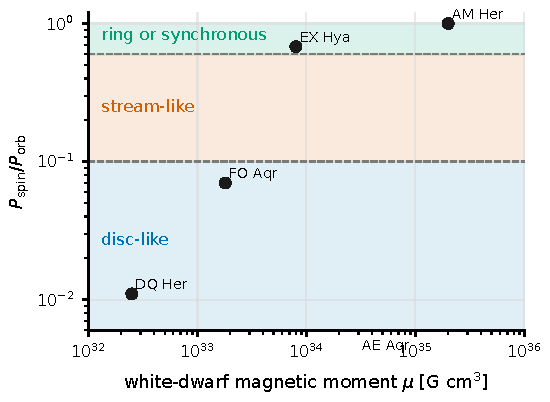
\includegraphics[width=0.78\linewidth]{figures/generated/chapter_11/ch11_magnetic_cv_flow_map.pdf}
\caption{The accretion flow of a magnetic cataclysmic variable is determined mainly by the white dwarf's magnetic moment and the speed of its rotation relative to the orbit. Low-\(P_{\rm spin}/P_{\rm orb}\) systems tend to form disk-like flows, the intermediate region often shows magnetically controlled flows, and near-synchronous or high-ratio systems shift toward ring, stream, or polar-system geometries; these geometries directly change the light-curve phase, circular polarization, and correlation functions.}
\label{fig:e18-mcv-map}
\end{figure}

The falling flow releases gravitational potential energy, turning it into light. The order of magnitude is given by the depth of the potential well times the mass flow rate:

\begin{equation}
  L_{\rm acc}\simeq \frac{GM\dot M}{R_{\rm WD}}
  \simeq 1.0\times10^{33}\,\mathrm{erg\,s^{-1}}
  \left(\frac{M}{0.8\,M_\odot}\right)
  \left(\frac{\dot M}{10^{-10}M_\odot\,\mathrm{yr^{-1}}}\right)
  \left(\frac{8\times10^8\,\mathrm{cm}}{R_{\rm WD}}\right).
  \label{eq:e18-lacc}
\end{equation}
\begin{formulaexplain}
\(L_{\rm acc}\): the accretion luminosity (\(\mathrm{erg\,s^{-1}}\)), equal to the gravitational potential energy released per unit time \(GM\dot M/R\). It gives the order of magnitude of the photon rate available in such systems; the optical receives only a portion of it.
\end{formulaexplain}

This luminosity is a blend of various components: the accretion disk, hot spots near the magnetic poles, the columnar shock region, the illuminated white-dwarf surface, and \emph{cyclotron emission}. Here we connect to a pedagogical focus of this chapter: how a strong field writes polarization into the light. A charged electron in a magnetic field spirals around the field lines, and the angular frequency of that spiraling is the cyclotron frequency
\[
  \omega_c=\frac{eB}{m_e c},
  \qquad
  \hbar\omega_c\approx 11.6\,\mathrm{keV}\left(\frac{B}{10^{12}\,\mathrm{G}}\right).
\]
An electron going in circles is an accelerating charge and radiates; the radiation is concentrated at \(\omega_c\) and its harmonics. For magnetic white dwarfs with \(B\sim10\)--\(200\,\mathrm{MG}=10^7\)--\(2\times10^8\,\mathrm{G}\), the fundamental photon energy \(\hbar\omega_c\sim0.1\)--\(2\,\mathrm{eV}\), plus several harmonics, falls right in the near-infrared to optical: this is why the optical light curve of a polar shows a string of ``cyclotron humps.'' The key point: an electron circling the field lines radiates with natural \emph{polarization}: looking along the field lines you see circular polarization, looking sideways you see linear polarization. So polarization becomes the probe that \emph{picks out} the cyclotron component from the disk light and the blackbody light. (Replace the non-relativistic cyclotron radiation with relativistic electrons, and it is the synchrotron radiation discussed in Chapter~\ref{chap:e16}; the two are the two faces of the same mechanism in different energy bands.)

How does polarization read the geometry? Two empirical rules are very useful. First, if the \emph{sign} of the circular polarization flips with rotation phase, it usually means the line of sight has swept across different magnetic poles, or the projected field direction has changed sign. Second, if the linear-polarization peak and the total light-curve peak are \emph{not synchronous}, it says the ``brightest region'' and the ``region of most special field geometry'' are not the same patch: the intensity peak comes from shock-region heating, while the polarization peak comes from field projection.

How should these phase modulations be quantified in the event table? Bin the photons by white-dwarf rotation phase \(\phi_s\), and within each phase window compute the second-order intensity correlation (the \(g^{(2)}\) of Chapter~\ref{chap:e08}):

\begin{equation}
  g^{(2)}_{\phi_s}(\tau)=
  \frac{\langle I_{\phi_s}(t)\,I_{\phi_s}(t+\tau)\rangle}
       {\langle I_{\phi_s}(t)\rangle^2}.
  \label{eq:e18-g2phi}
\end{equation}
\begin{formulaexplain}
\(g^{(2)}_{\phi_s}(\tau)\): the second-order intensity correlation within a fixed rotation-phase window \(\phi_s\); \(I_{\phi_s}\): the count rate within that window. It extracts the ``short-term memory'' at delay \(\tau\) of the same magnetic pole or the same segment of accretion flow.
\end{formulaexplain}

The reading must be careful about timescales. If \(\tau\) is milliseconds to seconds, the structure of \(g^{(2)}\) may come from shock-region cooling, magnetically controlled clumps, or purely spurious signal from detector dead time; if \(\tau\) is tens of seconds to minutes, it is more like classical flickering or atmospheric transparency fluctuations than the compact source itself. And an iron rule: the average in \(\eqref{eq:e18-g2phi}\) \emph{must} be taken within the same phase window, the same energy band, and the same polarization channel, or else the orbital modulation will be mistaken for short-term correlation: this is exactly the weight the phrase ``phase-resolved'' carries.


\section{Neutron Stars: How the Magnetosphere Is Sliced into a Phase Event Table}
\label{sec:e18-nsphase}

A neutron star is an order of magnitude smaller still than a white dwarf: the radius is only \(10\)--\(14\,\mathrm{km}\), while the mass is often \(1.2\)--\(2.2\,M_\odot\). Such a small object spins extremely fast and has an extremely strong field, so its magnetosphere is ``sliced'' by rotation into a set of natural phase coordinates. The most basic boundary line is the light-cylinder radius: the place where the linear velocity of rigid corotation exactly reaches the speed of light:

\begin{equation}
  R_{\rm LC}=\frac{c}{\Omega}=\frac{cP}{2\pi}
  \simeq 1.6\times10^3\,\mathrm{km}
  \left(\frac{P}{33\,\mathrm{ms}}\right).
  \label{eq:e18-rlc}
\end{equation}
\begin{formulaexplain}
\(R_{\rm LC}\): the light-cylinder radius; \(P\): the rotation period; \(\Omega=2\pi/P\): the angular velocity. Here ``rigidly corotating with the star'' would require reaching the speed of light, so it is the outermost boundary that open field lines, particle acceleration, and high-energy radiation can be organized within.
\end{formulaexplain}

The derivation is one sentence: set the corotation linear velocity \(v=\Omega r\) equal to \(c\), and solve for \(r=c/\Omega=cP/2\pi\). The order of magnitude is quite vivid: the Crab pulsar has \(P\simeq33\,\mathrm{ms}\), light cylinder about \(1600\,\mathrm{km}\); millisecond pulsars have \(P\simeq1.5\)--\(10\,\mathrm{ms}\), light cylinder only tens to hundreds of km; a magnetar has \(P\simeq2\)--\(12\,\mathrm{s}\), light cylinder up to \(10^5\,\mathrm{km}\) and beyond. Within \(R_{\rm LC}\) the field lines are closed and corotate with the star; beyond it they must open, and particles accelerate and radiate along the open field lines. The discovery of pulsars and the interpretation as ``rotating neutron stars'' established this picture, and the Crab further linked rotational energy loss to a supernova remnant \citep{1968Natur.217..709H,1968Natur.218..731G,1968Natur.219..145P,1972ApJ...175..217B}. Figure~\ref{fig:e18-lc} draws the linear growth of the light cylinder with period and the Crab-type phase profile.

\begin{figure}[tbp]
\centering
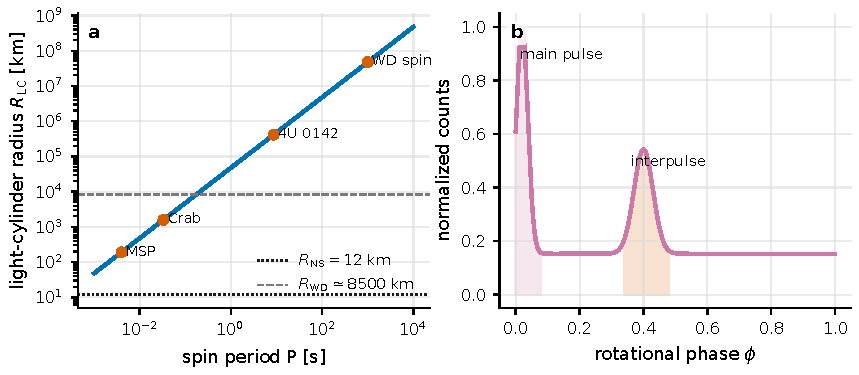
\includegraphics[width=0.94\linewidth]{figures/generated/chapter_11/ch11_light_cylinder_phase.pdf}
\caption{The light-cylinder radius increases linearly with rotation period. A millisecond pulsar's light cylinder is only tens to hundreds of km, the Crab's about \(1.6\times10^3\,\mathrm{km}\), and a magnetar's can reach \(10^5\,\mathrm{km}\) and beyond. The right panel is a Crab-type phase-folded profile, where the phase windows of the main pulse and interpulse determine which photons enter the subsequent intensity correlation or polarization statistics.}
\label{fig:e18-lc}
\end{figure}

How strong is the field? We cannot measure the neutron-star surface, but we can infer it from its ever-slowing rotation. A magnetized rotating body is like an antenna, radiating a magnetic-dipole wave outward and carrying away energy, so the rotation slows. The intermediate bridge for this step is the magnetic-dipole radiation formula: a dipole of magnetic moment \(m=B R^3\), rotating at angular velocity \(\Omega\), with the magnetic axis at angle \(\chi\) to the rotation axis, radiates the power (the classical Larmor formula generalized to a rotating magnetic dipole)
\[
  \dot E_{\rm dip}=\frac{B^2R^6\Omega^4\sin^2\chi}{6c^3}.
\]
Setting this radiative loss equal to the loss of rotational kinetic energy \(\dot E=I\Omega\dot\Omega\) (the next equation~\eqref{eq:e18-edot} will expand it), equating the two, solving for \(B\), then substituting the standard assumptions \(R=10\,\mathrm{km}\), \(I=10^{45}\,\mathrm{g\,cm^2}\), \(\sin\chi=1\), and converting \(\Omega=2\pi/P\), \(\dot\Omega=-2\pi\dot P/P^2\) into period, one tidies up the equatorial surface field

\begin{equation}
  B_{\rm dip}\simeq 3.2\times10^{19}\,(P\dot P)^{1/2}\,\mathrm{G}.
  \label{eq:e18-bdip}
\end{equation}
\begin{formulaexplain}
\(B_{\rm dip}\): the dipole field inferred from rotational slowdown (\(\mathrm{G}\)); \(P\) in seconds, \(\dot P\) (dimensionless \(\mathrm{s\,s^{-1}}\)) the rate of change of the period. It translates the ``spinning down'' in the timing data into a field scale.
\end{formulaexplain}

The numbers tell us how outrageous the neutron-star field is: ordinary young pulsars have \(B_{\rm dip}\sim10^{11}\)--\(10^{13}\,\mathrm{G}\), and magnetars can reach \(10^{14}\)--\(10^{15}\,\mathrm{G}\); the Earth's field is only \(0.5\,\mathrm{G}\), and even the strongest laboratory steady-state field is only of order \(10^5\,\mathrm{G}\). This field is the stage behind vacuum birefringence. The rate of energy released by slowdown is

\begin{equation}
  \dot E = 4\pi^2 I\,\frac{\dot P}{P^3},
  \qquad
  I\simeq10^{45}\,\mathrm{g\,cm^2}.
  \label{eq:e18-edot}
\end{equation}
\begin{formulaexplain}
\(\dot E\): the rotational-energy loss rate (\(\mathrm{erg\,s^{-1}}\)); \(I\): the moment of inertia (about \(10^{45}\,\mathrm{g\,cm^2}\)). It is the total energy budget for the pulsar to drive magnetospheric radiation and the nebula.
\end{formulaexplain}

Derivation: the rotational kinetic energy \(E=\tfrac12 I\Omega^2=2\pi^2 I/P^2\), differentiated in time gives \(\dot E=-4\pi^2 I\dot P/P^3\) (the positive sign denoting the loss rate). The Crab's \(\dot E\sim10^{38}\,\mathrm{erg\,s^{-1}}\) is enough to light up the pulses from radio to \(\gamma\)-rays and the entire Crab nebula \citep{1984ApJ...283..279H,1992ApJ...397..187B,2001A&A...378..918K,2008ApJ...680.1378H}.

Now send the photons into the phase coordinate. Each photon first receives a barycentric correction (subtracting the arrival-time difference caused by the Earth's orbital motion), then is folded into a phase using the timing ephemeris:

\begin{equation}
  \phi_i=
  \left[
  \nu(t_i-t_0)+\tfrac12\dot\nu(t_i-t_0)^2
  +\tfrac16\ddot\nu(t_i-t_0)^3+\cdots
  \right]\bmod 1 .
  \label{eq:e18-fold}
\end{equation}
\begin{formulaexplain}
\(\phi_i\): the rotation phase of the \(i\)-th photon (\(0\)--\(1\)); \(t_i\): its barycentric arrival time; \(\nu=1/P\) and \(\dot\nu,\ddot\nu\): the rotation frequency and its derivatives. Taking \(\bmod\,1\) rolls the long arrival-time table into a single cycle of phase.
\end{formulaexplain}

Term by term: \(t_i\) is the barycentric time (seconds), \(t_0\) is the reference epoch, \(\nu\) describes the basic rotation, \(\dot\nu\) describes the slowdown, and \(\ddot\nu\) describes higher-order terms such as post-glitch recovery. This step rolls ``a long string of arrival times'' into ``one cycle of phase from \(0\) to \(1\),'' and superposing many cycles gives a high-signal-to-noise pulse profile (Figure~\ref{fig:e18-lc}, right). The Crab's main-pulse width occupies only about \(0.04\)--\(0.05\) in phase, and radio giant pulses can be as narrow as microseconds. Interestingly: picking out the rotation cycles in which giant radio pulses occur, the optical main pulse is on average enhanced by about \(3\%\), while the pulse shape and arrival phase are essentially unchanged; the energy-resolved photon counting of ARCONS further shows that the optical enhancement corresponding to early-arriving giant radio pulses can reach a dozen to a couple dozen percent \citep{2003Sci...301..493S,2013ApJ...779L..12S}. These results connect the coherent radio bursts and the incoherent optical radiation to the same portion of magnetospheric plasma, a connection visible only when the radio and the optical are placed in the \emph{same phase event table}.

With the phase coordinate in hand, one can do phase-resolved second-order correlation, comparing the synchronous fluctuations of different energy bands, polarizations, or telescopes at the same pulse phase:

\begin{equation}
  g^{(2)}_{ab}(\tau\mid\Phi)=
  \frac{\langle n_a(t,\Phi)\,n_b(t+\tau,\Phi)\rangle}
       {\langle n_a(t,\Phi)\rangle\langle n_b(t,\Phi)\rangle},
  \label{eq:e18-g2ab}
\end{equation}
\begin{formulaexplain}
\(g^{(2)}_{ab}(\tau\mid\Phi)\): the cross-correlation of channels \(a\) and \(b\) within the phase window \(\Phi\); \(n_a,n_b\): the counts of the two channels. \(a,b\) can be energy bands, polarizations, or different telescopes, used to examine synchronicity at the same pulse phase.
\end{formulaexplain}

For a bright source like the Crab, \(\tau\) can be pushed to microseconds to milliseconds, truly approaching single-pulse statistics; for fainter optical pulsars, the first thing achievable is usually still only the luminosity and polarization stacking within a phase window, still far from pulse-by-pulse correlation \citep{1996ApJ...468..779M,2000ApJ...537..861S,2009MNRAS.397..103S}. When \(a,b\) here point to different telescopes, \(\eqref{eq:e18-g2ab}\) connects directly to the intensity interferometry of Chapter~\ref{chap:e10}, only now each \(g^{(2)}\) hangs on a rotation-phase label.


\section{Strong-Field Polarization: The Imprint of Vacuum Birefringence and QED Strong-Field Effects}
\label{sec:e18-qed}

This section walks to the most ``quantum'' place in the chapter's physics. In classical electrodynamics the vacuum is empty, bends no light, and separates no polarization. But quantum electrodynamics (QED) says: the vacuum in fact seethes with virtual electron--positron pairs, and a strong field \emph{polarizes} them, turning the vacuum into a medium with a preferred polarization direction, birefringent like a calcite crystal. This effect is called vacuum birefringence. When does it grow strong? The yardstick is the QED critical field:

\begin{equation}
  B_Q=\frac{m_e^2c^3}{e\hbar}=4.414\times10^{13}\,\mathrm{G}.
  \label{eq:e18-bq}
\end{equation}
\begin{formulaexplain}
\(B_Q\): the QED critical field. At this field strength, the cyclotron energy of the lowest Landau level of the electron already approaches its rest energy \(m_ec^2\), and the quantum magnetic effect is no longer a small correction. A magnetar surface \(B\) approaches or even exceeds \(B_Q\).
\end{formulaexplain}

The physical meaning of \(B_Q\) is worth savoring: set \(\hbar\omega_c=\hbar eB/(m_ec)\) equal to the electron rest energy \(m_ec^2\), and the solution is precisely \(B=m_e^2c^3/(e\hbar)=B_Q\). That is to say, when the field is so strong that ``the quantum energy of one electron cyclotron loop equals its entire rest mass,'' the quantum structure of the vacuum can no longer be ignored. A magnetar surface \(B\sim10^{14}\)--\(10^{15}\,\mathrm{G}\) is an order of magnitude larger than \(B_Q\): vacuum birefringence here is no armchair theorizing.

When \(B\ll B_Q\) and the photon energy is far below \(m_ec^2\), the Heisenberg--Euler effective theory gives the refractive-index difference between the two polarization normal modes (weak-field approximation):

\begin{equation}
  \Delta n\simeq\frac{\alpha_{\rm fs}}{30\pi}
  \left(\frac{B_\perp}{B_Q}\right)^2 ,
  \label{eq:e18-dn}
\end{equation}
\begin{formulaexplain}
\(\Delta n\): the refractive-index difference between the parallel and perpendicular polarization normal modes; \(B_\perp\): the field component perpendicular to the light ray; \(\alpha_{\rm fs}\simeq1/137\): the fine-structure constant. It grows as \(B_\perp^2\): double the field, and the birefringence quadruples.
\end{formulaexplain}

Note \(\Delta n\propto B_\perp^2\): the field is the ``accelerator'' of this effect, and it is stepped on hard. The magnetar surface field exceeds \(B_Q\), so the weak-field formula can no longer serve as an exact model, but it lays bare the crux: \emph{polarization is extremely sensitive to the strong field}. The two polarization modes propagate in the vacuum at slightly different speeds, accumulating a phase difference along the light path:

\begin{equation}
  \Delta\Phi(E)=\frac{E}{\hbar c}\int\Delta n(s)\,ds .
  \label{eq:e18-dphi}
\end{equation}
\begin{formulaexplain}
\(\Delta\Phi(E)\): the phase difference accumulated by the two polarization modes; \(E\): the photon energy; the integral runs along the light path \(s\). The higher the energy and the larger the \(\Delta n\) along the path, the stronger the polarization-propagation effect.
\end{formulaexplain}

This phase difference brings an observable consequence, called polarization freezing. Imagine photons setting out from different small patches on the magnetar surface, each patch with a different field direction and hence a different polarization direction. Without vacuum birefringence, these randomly oriented polarizations superposed would cancel each other, and the observed net polarization degree would be low. But with birefringence, as long as the propagation is adiabatic, the polarization vector \emph{locks} onto the local field direction and rotates slowly with the field, freezing out only at the far ``polarization-limiting radius.'' The result: the polarization directions from a large area of the stellar surface are ``combed'' into alignment by the field, cancellation is reduced, and the net polarization degree instead \emph{rises}. So \textbf{a high polarization degree is itself an indirect imprint of vacuum birefringence}. This picture comes from the combination of strong-field QED, magnetospheric propagation, and neutron-star surface radiation models \citep{1936ZPhy...98..714H,1971AnPhy..67..599A,2000MNRAS.311..555H,2002PhRvD..66b3002H,2003MNRAS.342..134H}. An X-ray polarimeter (such as IXPE) works at \(2\)--\(8\,\mathrm{keV}\), precisely to measure this polarization in this energy band.

So how exactly are ``polarization degree'' and ``polarization angle'' computed from the photons? This is the core tool shared by this chapter and Chapter~\ref{chap:e22}. An X-ray polarimeter measures an azimuthal angle (modulation angle) \(\eta_i\) for each photoelectric event, then accumulates many events into the Stokes parameters (the total intensity \(I\) below is the same symbol as, but a different quantity from, the moment of inertia \(I\) of~\eqref{eq:e18-edot}; do not confuse them):

\begin{equation}
  I=\sum_i w_i,\qquad
  Q=\sum_i w_i\cos 2\eta_i,\qquad
  U=\sum_i w_i\sin 2\eta_i .
  \label{eq:e18-stokes}
\end{equation}
\begin{formulaexplain}
\(I\): the total intensity; \(Q,U\): the two linear-polarization Stokes components; \(\eta_i\): the azimuthal angle of the \(i\)-th event; \(w_i\): the weight (including instrument modulation, background, and effective-area factors). The factor \(2\) in front of the angle reflects that polarization is ``undirected'': rotating \(180^\circ\) returns to itself.
\end{formulaexplain}

Why \(\cos2\eta\) rather than \(\cos\eta\)? Because polarization is an \emph{undirected line}: rotating the polarization direction by \(180^\circ\) is the same as not rotating it, so the physical quantity must have period \(2\eta\). Weighting and summing the azimuthal angles of a large number of events this way, the random directions cancel each other, and only the truly polarized direction leaves a net vector in \(Q,U\). From it we obtain the polarization degree and polarization angle:

\begin{equation}
  p=\frac{\sqrt{Q^2+U^2}}{I},\qquad
  \psi=\tfrac12\arctan2(U,Q).
  \label{eq:e18-pdop}
\end{equation}
\begin{formulaexplain}
\(p\): the linear polarization degree (\(0\)--\(1\)); \(\psi\): the polarization angle. The \emph{length} of the two-dimensional vector \((Q,U)\) gives the polarization strength, and its \emph{direction} (after dividing by 2) gives the polarization angle on the sky.
\end{formulaexplain}

Plug in a real number: optical polarization measurements of the isolated neutron star RX J1856.5\(-\)3754 gave \(p=16.43\%\pm5.26\%\), while the source itself is as faint as \(V\simeq25.5\); the foreground interstellar polarization and the instrument polarization must both be subtracted item by item. Such an elevated polarization degree, compared against thermal surface models, supports vacuum birefringence having reduced the polarization cancellation of different surface regions \citep{2015MNRAS.454.3254T,2016MNRAS.459.3585G,2017MNRAS.465..492M}. Figure~\ref{fig:e18-stokes} shows how the rotating magnetic geometry projects the polarization into phase curves of \(Q/I\), \(U/I\) and a track on the Q--U plane.

\begin{figure}[tbp]
\centering
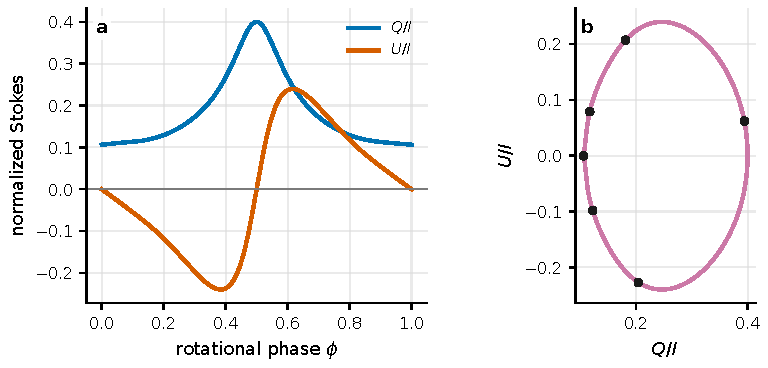
\includegraphics[width=0.92\linewidth]{figures/generated/chapter_11/ch11_stokes_qu_track.pdf}
\caption{The rotating magnetic geometry projects the polarization-angle variation into phase curves of \(Q/I\) and \(U/I\). The left panel shows the two Stokes components given by the same phase event table, and the right panel shows the corresponding Q--U track; the shape of the track exposes geometric degeneracy and instrument crosstalk better than the polarization degree alone.}
\label{fig:e18-stokes}
\end{figure}

How does the polarization angle swing with phase? To first approximation one uses the rotating vector model:

\begin{equation}
  \tan(\psi-\psi_0)=
  \frac{\sin\alpha\,\sin(\phi-\phi_0)}
       {\sin\zeta\cos\alpha-\cos\zeta\sin\alpha\cos(\phi-\phi_0)} .
  \label{eq:e18-rvm}
\end{equation}
\begin{formulaexplain}
\(\psi\): the polarization angle; \(\alpha\): the angle between the magnetic axis and the rotation axis; \(\zeta\): the angle between the line of sight and the rotation axis; \(\phi\): the rotation phase; \(\psi_0,\phi_0\): the zero points. It translates ``the S-shaped swing of the polarization angle with phase'' into the geometric orientation of the magnetosphere.
\end{formulaexplain}

This equation was first used for the polarization geometry of radio pulsars: it is purely the spherical trigonometry of ``projecting the field lines onto the sky.'' But in magnetar X-rays, it is only a low-dimensional geometric skeleton, because surface radiation, resonant cyclotron scattering, and vacuum birefringence together rewrite \(p(E,\phi)\) and \(\psi(E,\phi)\), making the measured polarization far richer than pure geometry \citep{1969ApL.....3..225R,2018ApJ...854...98W,2011ApJ...730..131F}.

Consider a real example that twines these clues together: the magnetar 4U 0142+61 (Figure~\ref{fig:e18-biref}). IXPE in the full \(2\)--\(8\,\mathrm{keV}\) band saw a linear polarization degree of \(12\%\pm1\%\), but split by energy band the story is more remarkable: low energy \(2\)--\(4\,\mathrm{keV}\) polarization degree \(14\%\pm1\%\), high energy \(5.5\)--\(8\,\mathrm{keV}\) soaring to \(41\%\pm7\%\), while in the intermediate range near \(4\)--\(5\,\mathrm{keV}\) the polarization degree drops to the sensitivity floor and the polarization angle even flips by about \(90^\circ\). This \(90^\circ\) flip is the key fingerprint: it means the two polarization normal modes (the O mode and the X mode) ``switch shifts'' at this energy: at low energy one mode dominates, at high energy the other, and at the crossover the two cancel and the direction turns around. The source's rotation period is \(P=8.69\,\mathrm{s}\), the field \(B\sim10^{14}\,\mathrm{G}\), the soft X-ray has a blackbody component with \(kT\sim0.5\)--\(1\,\mathrm{keV}\), and the hard tail extends to tens or even hundreds of keV. In explaining this dataset, the low-energy O mode, the hard-tail X mode, a surface condensate or thin atmosphere, and resonant Compton scattering may all participate; a \emph{single} high-polarization point alone is not yet enough to determine vacuum birefringence on its own, and requires cross-validation across energy, phase, and multiple sources \citep{2022Sci...378..646T,2023A&A...674L..10C,2023MNRAS.519.3681F}.

\begin{figure}[tbp]
\centering
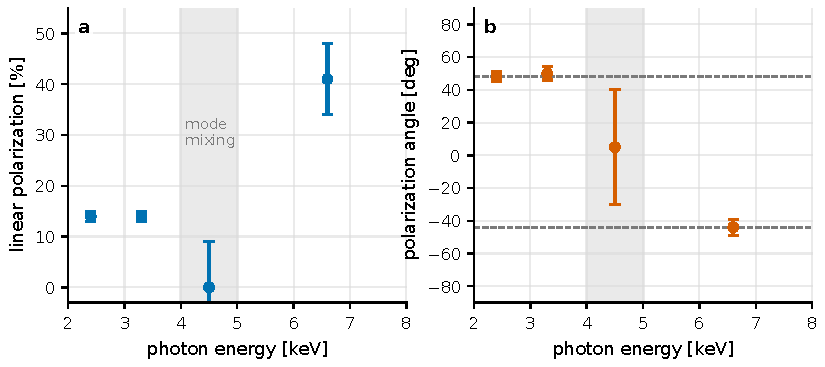
\includegraphics[width=0.92\linewidth]{figures/generated/chapter_11/ch11_birefringence_energy.pdf}
\caption{The IXPE result on the magnetar 4U 0142+61 can be viewed as a switching of the two polarization normal modes with energy. Low energy \(2-4\,\mathrm{keV}\) polarization degree about \(14\%\), high energy \(5.5-8\,\mathrm{keV}\) rising to about \(41\%\), while near \(4-5\,\mathrm{keV}\) the polarization degree approaches the minimum detectable polarization and the polarization angle flips by about \(90^\circ\).}
\label{fig:e18-biref}
\end{figure}

Bring this section back to the main thread of the book. Each step above (measuring \(\eta_i\), accumulating the Stokes parameters, computing \(p\) and \(\psi\), binning by phase and energy) is in essence \textbf{doing intensity/count statistics on the polarization channel}. It is the same family of tools as the \(g^{(2)}\) of Chapter~\ref{chap:e08} and the intensity interferometry of Chapter~\ref{chap:e10}: only now the ``two telescopes'' or ``two instants'' are replaced by ``two polarization bases.'' Chapter~\ref{chap:e22} will formally develop this ``polarization quantum channel,'' discussing its use in the search for new physics such as dark matter and axions; the magnetar birefringence here is the cleanest training ground for this channel on strong-field objects.


\section{Surface and Atmospheric Radiation: How Hot-Spot Light Curves Infer the Neutron-Star Radius}
\label{sec:e18-hotspot}

Finally, we return to the old problem of ``what to do when we cannot resolve,'' but switched to the neutron star, the answer is especially beautiful. The neutron-star radius cannot be measured through the angular diameter (Section~\ref{sec:e18-angsize} said it is even smaller than a white dwarf), yet it can be measured to \(\sim1\,\mathrm{km}\) precision: relying not on spatial resolution but on \emph{light-curve shape + energy spectrum + general relativity}. The core quantity is the compactness:

\begin{equation}
  u=\frac{2GM}{Rc^2}
  \simeq 0.345
  \left(\frac{M}{1.4\,M_\odot}\right)
  \left(\frac{12\,\mathrm{km}}{R}\right).
  \label{eq:e18-compact}
\end{equation}
\begin{formulaexplain}
\(u\): the compactness, equal to the ratio of the Schwarzschild radius \(2GM/c^2\) to the true radius \(R\) (dimensionless). The larger \(u\), the stronger the gravitational bending of light, and the more easily the amplitude of the hot-spot light curve is smoothed away.
\end{formulaexplain}

The physical picture: the neutron-star surface often has one or two spots hotter than their surroundings (hot spots near the magnetic poles). As the star rotates, the hot spot sweeps across the line of sight and we see pulsation. But the neutron star's gravity is strong enough to \emph{bend} light: a hot spot that has rotated to the far side and should be invisible has its emitted light dragged back into our line of sight by gravity. The larger the compactness, the harder the bending, and the more the far-side spot can ``leak'' through, so the pulse troughs are raised and the amplitude flattened. Writing this bending effect as a useful approximation, relating the emission angle \(\alpha\) at which the photon leaves the surface (here \(\alpha\) is the geometric emission angle, the same symbol as, but a different quantity from, the fine-structure constant \(\alpha_{\rm fs}\) earlier and the magnetic-axis angle \(\alpha\) in the rotating vector model) and the central angle \(\psi\) of the hot spot relative to the line of sight (here \(\psi\) is the spatial angular distance, not the polarization angle \(\psi\) of~\eqref{eq:e18-pdop} and~\eqref{eq:e18-rvm}):

\begin{equation}
  \cos\alpha\simeq u+(1-u)\cos\psi .
  \label{eq:e18-bending}
\end{equation}
\begin{formulaexplain}
\(\alpha\): the emission angle of the photon leaving the stellar surface relative to the normal; \(\psi\): the angular distance of the hot-spot center relative to the line of sight. This linear approximation writes ``whether a spot is still visible after bending'' as a simple function of the compactness \(u\).
\end{formulaexplain}

It applies to the Schwarzschild exterior spacetime and scaling estimates from slow to moderate rotation; a real millisecond pulsar must further add Doppler boosting, aberration, time delay, stellar oblateness, and atmospheric beaming. Figure~\ref{fig:e18-hotspot} shows that at low compactness the pulse amplitude is large, and at high compactness the trough is raised: radius inference exploits exactly this change in profile \citep{2002ApJ...566L..85B,2019AIPC.2127b0008W}.

\begin{figure}[tbp]
\centering
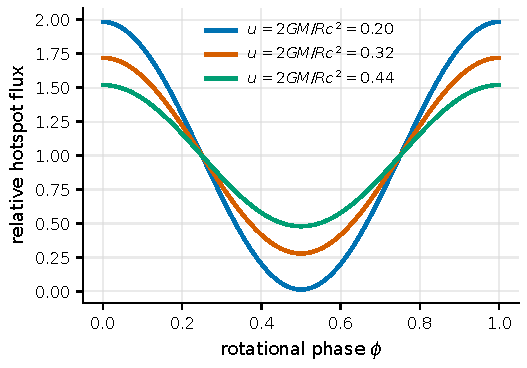
\includegraphics[width=0.78\linewidth]{figures/generated/chapter_11/ch11_hotspot_lightcurve.pdf}
\caption{The hot-spot light curve is very sensitive to compactness. At low compactness, the spot's contribution vanishes quickly after it rotates to the far side, and the pulse amplitude is large; at high compactness, gravitational light bending makes a larger area of the surface visible, and the light-curve trough is raised. Radius inference exploits this profile change and fits it jointly with mass, inclination, hot-spot position, and atmospheric beaming.}
\label{fig:e18-hotspot}
\end{figure}

How to turn this physics into a measurement of \(M,R\)? The key is to realize: all we have in hand is an \emph{event table}: each X-ray photon carries an energy and a rotation phase. Compute the astrophysical model (hot-spot geometry + atmosphere + gravitational bending) forward into ``how many photons there should be in each energy channel and each phase bin,'' then compare with the measurement. The expected count in the \(j\)-th energy channel and \(k\)-th phase bin is
\begin{equation}
  \lambda_{jk}(\Theta)=
  T\int dE\,R_j(E)\,
  \left[F_E(\phi_k;\Theta)+B_E\right].
  \label{eq:e18-lambda}
\end{equation}
\begin{formulaexplain}
\(\lambda_{jk}\): the expected count in energy channel \(j\), phase bin \(k\); \(T\): the exposure time; \(R_j(E)\): the instrument response (effective area + energy redistribution); \(F_E\): the hot-spot model flux; \(B_E\): the background. \(\Theta\) holds all the parameters: \(M,R\), distance, inclination, hot-spot position, etc. It translates the astrophysical model into the expected number of events in the detector.
\end{formulaexplain}

The parameter vector \(\Theta\) is packed with \(M,R\), distance, observer inclination, hot-spot latitude and longitude, hot-spot angular radius, temperature, and atmospheric parameters, a whole set. The measured count will of course not exactly equal \(\lambda_{jk}\); it follows Poisson statistics (Chapter~\ref{chap:e03}): given the expectation \(\lambda\), the probability of observing \(N\) is \(e^{-\lambda}\lambda^N/N!\). Multiplying the probabilities over all energy channels and phase bins and taking the logarithm gives the Poisson log-likelihood:
\begin{equation}
  \ln\mathcal{L}(\Theta)=
  \sum_{j,k}\left[
  N_{jk}\ln\lambda_{jk}(\Theta)-\lambda_{jk}(\Theta)-\ln(N_{jk}!)
  \right].
  \label{eq:e18-lnl}
\end{equation}
\begin{formulaexplain}
\(\ln\mathcal{L}\): the Poisson log-likelihood; \(N_{jk}\): the measured count. Multiplying \(e^{-\lambda}\lambda^N/N!\) over all \((j,k)\) and taking the logarithm gives it. Finding the radius means finding a set of \(\Theta\) that makes all \(\lambda_{jk}\) fit the event table best.
\end{formulaexplain}

The derivation needs only one step: \(\ln\prod_{jk}\dfrac{e^{-\lambda_{jk}}\lambda_{jk}^{N_{jk}}}{N_{jk}!}=\sum_{jk}\big(-\lambda_{jk}+N_{jk}\ln\lambda_{jk}-\ln N_{jk}!\big)\). The last term \(\ln N_{jk}!\) contains no parameters and is a constant in the fit, which may be dropped. What remains is the objective to be \emph{maximized}: this is exactly the general paradigm of event-table modeling of Chapter~\ref{chap:e13}, only that the ``astrophysical model'' here is packed with gravitational bending and a strong-field atmosphere. The NICER radius measurements of PSR J0030+0451 and PSR J0740+6620 were done just this way: the J0740 analysis combined the NICER event table, the XMM-Newton imaging-spectroscopy background, and the mass and distance priors from radio timing, and Riley et al. obtained \(R=12.39^{+1.30}_{-0.98}\,\mathrm{km}\), \(M=2.072^{+0.067}_{-0.066}\,M_\odot\), while Miller et al. gave a constraint from a different method but consistent; the two independent analyses of J0030 further show that the hot-spot geometry may carry a complex multipole field structure \citep{2019ApJ...887L..21R,2019ApJ...887L..24M,2021ApJ...918L..27R,2021ApJ...918L..28M}. Appreciate the weight of this: we did not resolve a \(12\,\mathrm{km}\) sphere (that would require nanoarcsecond resolution), yet we measured its radius to the kilometer level: purely by time, energy, and gravitational optics, ``folding'' the spatial information into the event table.


\section{Chapter Summary}
\label{sec:e18-summary}

\begin{itemize}
\item \textbf{Compact objects are held up by quantum degeneracy, and are therefore ``extremely small.''} A white dwarf is held up against gravity by electron degeneracy pressure (\(\eqref{eq:e18-pnr}\), \(\eqref{eq:e18-per}\)), showing a ``heavier means smaller'' mass--radius relation; but the angular diameter is only microarcseconds (\(\eqref{eq:e18-theta}\)), and the neutron star is smaller still, making single-aperture imaging hopeless: this hands the baton precisely to intensity interferometry (Chapter~\ref{chap:e10}) and the time/polarization channels.
\item \textbf{The magnetic field writes geometry into phase and polarization.} The ratio of the magnetospheric radius to the corotation radius of a magnetic white dwarf (\(\eqref{eq:e18-rm}\), \(\eqref{eq:e18-rco}\)) determines the accretion-flow morphology, and cyclotron radiation brings a selectable polarization signal; the light cylinder, dipole field, and rotational-energy loss of a neutron star (\(\eqref{eq:e18-rlc}\)--\(\eqref{eq:e18-edot}\)) slice the magnetosphere into a phase coordinate, read out by phase folding (\(\eqref{eq:e18-fold}\)).
\item \textbf{Vacuum birefringence is the imprint of strong-field QED on polarization.} A magnetar surface \(B\) approaches or even exceeds the critical field \(B_Q\) (\(\eqref{eq:e18-bq}\)), the vacuum becomes a birefringent medium (\(\eqref{eq:e18-dn}\)), combing the polarization everywhere on the stellar surface into alignment and raising the net polarization degree; the energy-dependent polarization degree and \(90^\circ\) polarization-angle flip of 4U 0142+61 are such an imprint, but require cross-validation across energy, phase, and multiple sources.
\item \textbf{Polarization measurement is essentially ``counting photons on polarization bases.''} Stokes accumulation (\(\eqref{eq:e18-stokes}\)), polarization degree and angle (\(\eqref{eq:e18-pdop}\)), and the rotating vector model (\(\eqref{eq:e18-rvm}\)) share the same lineage as the earlier \(g^{(2)}\), and are the direct precursor of the ``polarization quantum channel'' of Chapter~\ref{chap:e22}.
\item \textbf{If you cannot resolve, fold the spatial information into the event table.} The neutron-star radius is inferred from the hot-spot light curve + energy spectrum + gravitational bending (\(\eqref{eq:e18-compact}\)--\(\eqref{eq:e18-bending}\)), modeled with a Poisson-likelihood event table (\(\eqref{eq:e18-lambda}\), \(\eqref{eq:e18-lnl}\)), and NICER has already measured a \(12\,\mathrm{km}\) neutron star to the kilometer level.
\end{itemize}

\noindent\textbf{Questions to Ponder.}
(1) Why is a white dwarf ``heavier means smaller,'' while an ordinary main-sequence star is ``heavier means larger''? Think from the softening of the degeneracy-pressure exponent \(5/3\to4/3\).
(2) If vacuum birefringence \emph{did not exist}, would a magnetar's net polarization degree be higher or lower? Why can ``a high polarization degree'' serve as indirect evidence of birefringence?
(3) A neutron star's radius is only \(12\,\mathrm{km}\) and its angular diameter is far below the resolution limit of any telescope, yet we can measure its radius: in which dimension of the observational data is the measured ``information'' actually hidden?
